\documentclass[aspectratio=1610]{beamer}
\usetheme{Madrid}


\usepackage{amsmath}
\usepackage{amssymb}
\usepackage{listings}
\usepackage{booktabs}
\usepackage{multirow}
\usepackage{multirow}
\usepackage{lmodern}
\usepackage{xcolor}
\usepackage{float}
\lstset{
  language=Python,  %代码语言使用的是matlab
  % frame=shadowbox, %把代码用带有阴影的框圈起来
  rulesepcolor=\color{red!20!green!20!blue!20},%代码块边框为淡青色
  keywordstyle=\color{blue!90}\bfseries, %代码关键字的颜色为蓝色,粗体
  commentstyle=\color{red!10!green!70}\textit,    % 设置代码注释的颜色
  basicstyle=\footnotesize,
  showstringspaces=true,%不显示代码字符串中间的空格标记
  % numbers=left, % 显示行号
  % numberstyle=8pt,    % 行号字体
  % numberstyle=\color{green},
  stringstyle=\rmfamily\slshape\color[RGB]{128,0,0}, % 代码字符串的特殊格式
  breaklines=true, %对过长的代码自动换行
  extendedchars=false,  %解决代码跨页时,章节标题,页眉等汉字不显示的问题
  escapeinside=``,%代码中出现中文必须加上,否则报错
  texcl=true}

\lstset{breaklines}%自动将长的代码行换行排版

\lstset{extendedchars=false}%解决代码跨页时,章节标题,页眉等汉字不显示的问题

\usepackage{textcomp}
% \usepackage[margin=1in]{geometry}
\usepackage{pythonhighlight}
% \usepackage{minted}
\usepackage[backend=bibtex]{biblatex}
%\usepackage[style=authortitle,backend=biber]{biblatex}
\addbibresource{ResearchRabbit_Export_2022_10_20.bib}

\usepackage{algorithm}
\usepackage{algorithmic}
\renewcommand{\algorithmicrequire}{\textbf{Input:}}
\renewcommand{\algorithmicensure}{\textbf{Output:}}


\title[gates \& synthesis]{realization of three qubit-gates and synthesis Algorithm}
\author[Gcc]{Dingchao Gao}
\institute[ISCAS]{Institute of Software Chinese Academy of Sciences}

\begin{document}
\frame{\titlepage}

\begin{frame}
\frametitle{Table of Contents}
\tableofcontents[hideallsubsections]
\end{frame}


\section{Realization of a General Three-Qubit Quantum Gate}
\subsection{Two-Qubit Quantum Gates Recap}
\begin{frame}
\frametitle{Two-Qubit Quantum Gates Recap}
\begin{figure}
  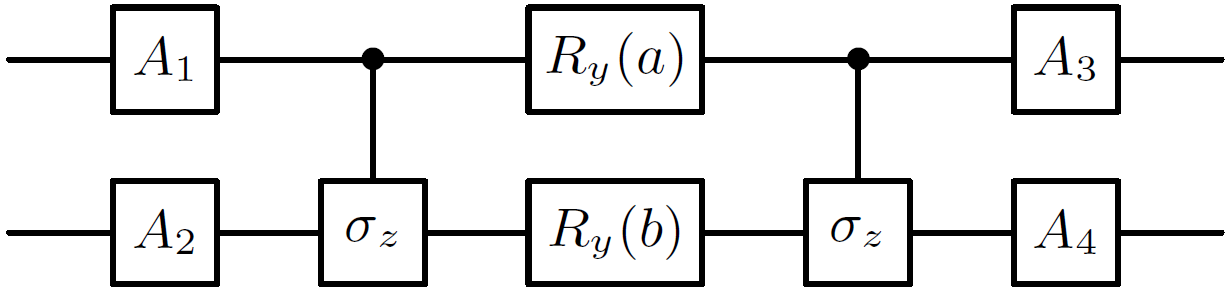
\includegraphics[width=\textwidth]{figure/two-qubit.png}
  \caption{Optimal Quantum Circuits for General Two-Qubit Gates are 15 single qubit gates and 3 CNOT gates\cite{two}}
\end{figure}
\end{frame}

\subsection{Introduction to Three-Qubit Quantum Gates}
\begin{frame}
\frametitle{Realization of Three-Qubit Quantum Gates}
\begin{itemize}
  \item universal gate family: $\{R_z,R_y,CNOT\}$
  \item basic idea: KAK Algorithm\cite{kak}, block-diagonal matrix
  \item results:98 single qubits and 40 CNOT gates
\end{itemize}
% introduce three qubit gates and the tools
\end{frame}

\subsection{Realization Techniques}
\subsubsection{Decomposition}
\begin{frame}
\frametitle{KAK Decomposition\cite{kak}}
any $SU(8)$ can be decomposed as
\begin{align}
  U&=K_{1} \exp \left(-i\left(\beta_{1} XXX+\beta_{2} YYX+\beta_{3} ZZX+\beta_{4} IIX\right)\right) K_{2}\\
  K_{1}&= P_{1}\exp \left(-i\left(\alpha_{1}XXX + \alpha_{2}YYZ + \alpha_{3}ZZZ\right)\right)P_{2},\\
  K_{1}&= P_{3}\exp \left(-i\left(\gamma_{1}XXX + \gamma_{2}YYZ + \gamma_{3}ZZZ\right)\right)P_{4}
\end{align}
% AKA results and step followed
\end{frame}
\frametitle{KAK Decomposition\cite{kak}}
\begin{figure}
  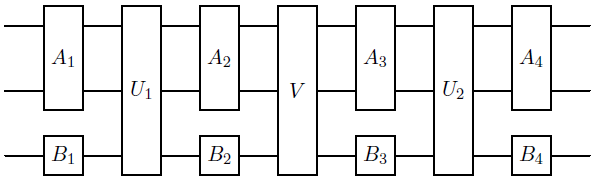
\includegraphics[width=\textwidth]{figure/three.png}
\end{figure}
% AKA results and step followed
\end{frame}
\subsubsection{Diagonalization}
\begin{frame}
\frametitle{Diagonalization}
...
% how and results figure
\end{frame}

\subsubsection{Block-Diagonalization}
\begin{frame}
\frametitle{Block-Diagonalization}
...
% result and way
\end{frame}

\subsubsection{Counter}
\begin{frame}
\frametitle{Counter}
...
%  the whole number
\end{frame}

\subsection{Later Work}
\begin{frame}
\frametitle{Later Work}
...
% the later AKA
\end{frame}

\section{QFAST Algorithm}

\subsection{Top-Down vs Bottom-Up Synthesizers}
\begin{frame}
\frametitle{Top-Down vs Bottom-Up Synthesizers}
...
% figure here
\end{frame}

\subsection{Introduction to QFAST Algorithm}
\begin{frame}
\frametitle{Introduction to QFAST Algorithm}
...
% work flow here
\end{frame}

\subsection{Gate Representation}
\begin{frame}
\frametitle{Gate Representation}
...
%  result formula
\end{frame}

\subsection{Cost Function for Optimization}
\begin{frame}
\frametitle{Cost Function for Optimization}
...
% function here and how to optimize
\end{frame}

\subsection{Comparison with Other Algorithms}
\begin{frame}
\frametitle{Comparison with Other Algorithms}
...
% how to compare and the metrics
\end{frame}
\begin{frame}
\frametitle{Comparison results}
\end{frame}
\subsection{Limitations}
\begin{frame}
\frametitle{Limitations}
...
% limitation here
\end{frame}

\section{Conclusion}
\begin{frame}
\frametitle{Summary}
...
% summary something
\end{frame}

\section{References}
\begin{frame}[noframenumbering,allowframebreaks,t]
	\frametitle{references}
	\printbibliography
\end{frame}
\begin{frame}
  \centering
  \Huge{END\\Thank you}
\end{frame}

\end{document}
